\documentclass[tikz]{standalone}

\usepackage{tikz}
\usetikzlibrary{arrows.meta}
\newcommand{\myarrow}{Latex[width=3mm]}
\newcommand\irregularcircle[2]{% radius, irregularity
  \pgfextra {\pgfmathsetmacro\len{(#1)+rand*(#2)}}
  +(0:\len pt)
  \foreach \a in {10,20,...,350}{
    \pgfextra {\pgfmathsetmacro\len{(#1)+rand*(#2)}}
    -- +(\a:\len pt)
  } -- cycle
}

\begin{document}
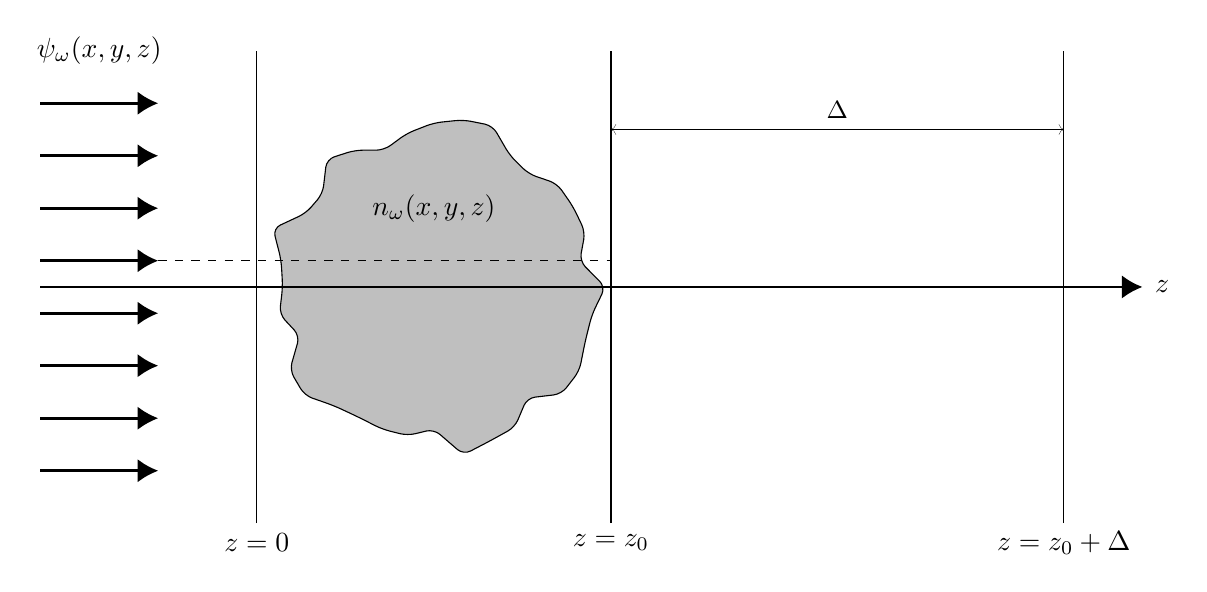
\begin{tikzpicture}
  % General frame is (0,0) to (10, 6)
    
  % Incoming waves
  \node (iw) at (0.75, 6) {$\psi_{\omega}(x,y,z)$};
  \draw[-\myarrow, line width=1.0pt] (0, 0.666) -- (1.5, 0.666);
  \draw[-\myarrow, line width=1.0pt] (0, 1.333) -- (1.5, 1.333);
  \draw[-\myarrow, line width=1.0pt] (0, 2) -- (1.5, 2);
  \draw[-\myarrow, line width=1.0pt] (0, 2.666) -- (1.5, 2.666);
  \draw[-\myarrow, line width=1.0pt] (0, 3.333) -- (1.5, 3.333);
  \draw[-\myarrow, line width=1.0pt] (0, 4) -- (1.5, 4);
  \draw[-\myarrow, line width=1.0pt] (0, 4.666) -- (1.5, 4.666);
  \draw[-\myarrow, line width=1.0pt] (0, 5.333) -- (1.5, 5.333);        

  % object
  \coordinate (center) at (5,3);
  \draw[fill=gray!50, rounded corners=1mm] (center) \irregularcircle{2cm}{2mm};
  \node (obj) at (5, 4) {$n_{\omega}(x,y,z)$};
  \draw[dashed] (1.5, 3.333) to (7.25, 3.333);  % projection line

  % optical axis
  \draw[-\myarrow, line width=1pt] (0,3) -- (14,3);
  \node (z) at (14.25,3) {$z$};

  % planes
  \draw (2.75,0) -- (2.75,6);
  \node (enter) at (2.75, -0.25) {$z=0$};
  \draw (7.25,0) -- (7.25,6);
  \node (exit) at (7.25, -0.25) {$z=z_0$};
  \draw (13, 0) -- (13, 6);
  \node (detect) at (13, -0.25) {$z = z_0 + \Delta$};

  % Delta label
  \draw[<->,line width = 0.1pt] (7.25, 5) -- (13, 5);
  \node (delta) at (10.125, 5.25) {\small$\Delta$};
  
\end{tikzpicture}
\end{document}